\documentclass[table]{article}
\usepackage[utf8]{inputenc}
\usepackage{amsmath}
\usepackage{framed}
\usepackage{tikz}
\usepackage{pgfplots}
\usepackage{relsize}
\pgfplotsset{compat=newest}
\title{%
    ECN 1101 - Introductory Maths - Semester 1 2021 \\
    \large Lecture Notes 2 - Application of Straight Line Geometry \\
}
\author{Lecturer: Anand Persaud \\ "Transliterator": Simeon Chester \\}
\date{2021-11-06}
\begin{document}

\maketitle

\relscale{1.2}
\section*{Objectives}
To determine
\begin{enumerate}
    \item the linear demand equation or demand function
    \item the linear supply equation or supply function
    \item the equilibrium point/position
    \item other outcomes: interpreting the slopes etc.
\end{enumerate}

\section*{}
Consider the following schedules:

\marginpar[parnote-1]{\raggedright The highlighted row shows equilibirum}
\begin{table}[h]
    \begin{center}
        \begin{tabular}{l|c|r}
            \textbf{Prices} & \textbf{Demand Units} & \textbf{Supply Units} \\
            \hline
            10              & 1400                  & 200                   \\
            20              & 1200                  & 300                   \\
            30              & 1000                  & 400                   \\
            40              & 800                   & 600                   \\
            \rowcolor{green}
            50              & 600                   & 600                   \\
            60              & 400                   & 700                   \\
            70              & 200                   & 800                   \\
        \end{tabular}
    \end{center}
    \caption{\label{tab:table-1} Table showing the demand and supply units along with corresponding prices for an unknown product}
\end{table}
\begin{figure}[h]
    \begin{center}
        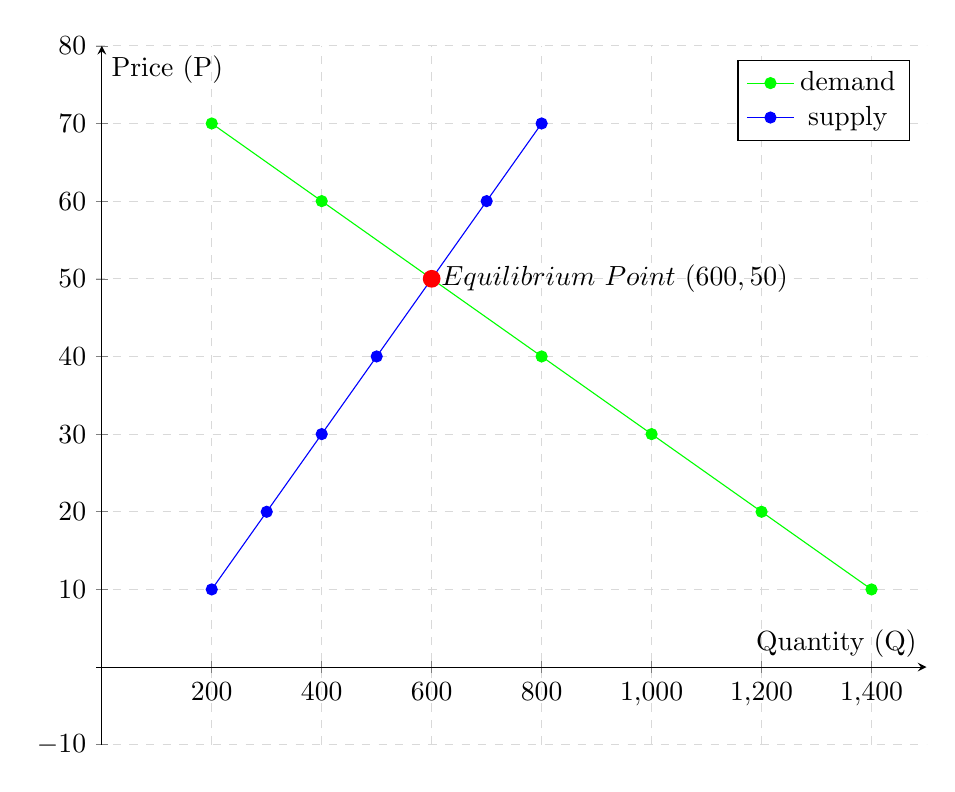
\begin{tikzpicture}
            \begin{axis}[
                    width = \linewidth,
                    xmin=-10,
                    xmax=1500,
                    ymin=-10,
                    ymax=80,
                    xlabel= Quantity (Q),
                    ylabel=Price (P),
                    grid=major,
                    grid style = {dashed, gray!30},
                    axis lines = center,
                ]

                \addplot[color=green,mark=*] coordinates {
                        (1400, 10)
                        (1200, 20)
                        (1000, 30)
                        (800, 40)
                        (600, 50)
                        (400, 60)
                        (200, 70)
                    };
                \addplot[color=blue,mark=*] coordinates {
                        (200, 10)
                        (300, 20)
                        (400, 30)
                        (500, 40)
                        (600, 50)
                        (700, 60)
                        (800, 70)
                    };

                \addplot[color=red, mark = *, mark size=3 pt] coordinates {
                        (600, 50)
                    };

                \node [right] at (axis cs: 600, 50) {$Equilibrium\ Point\ (600, 50)$};

                \legend{demand, supply}

            \end{axis}
        \end{tikzpicture}
        \caption{\label{Graph-1}Graph showing demand and supply units as a factor of price along with the market equilibrium point}
    \end{center}
\end{figure}
We should notice that as price increases, quantity demanded falls, while quantity supplied,
increases. At $10$\$ per unit, $1400$ are demanded while 200 units are supplied, at a higher price, say \$$60$
    per unit, $400$ units are demanded and supply increases.

    \section*{1. Determining the linear demand equation}

    Using: $$Q_{d} = mP+c$$ and $$m = \frac{Q_{2}-Q{1}}{P_{2}-P_{1}}$$ and choose any two ordered pairs from the demand schedule.
    Let us choose:

    $$
        \begin{aligned}
            \begin{pmatrix}
                20 \ \ 1200 \\
                P_1 \ \ Q_1
            \end{pmatrix} and &
            \begin{pmatrix}
                70 \ \ 200 \\
                P_2 \ \ Q_2
            \end{pmatrix}
        \end{aligned}
    $$

    and properly assign each.

    $$m = \frac{200-1200}{70-20} = -20$$

    $$
        Q_d = -20P + c
    $$

    To find $c$, simply use any any $P$ and $Q$ pair from the schedule and plug it into the aforementioned equation found.

    Using
    $$
        \begin{pmatrix}
            20 \ \ 1200 \\
            P_1 \ \ Q_1 \\
        \end{pmatrix}
    $$
    we get
    $$
        \begin{aligned}
            Q_d         & = -20P + c   \\
            1200        & = -20(20)+c  \\
            -20(20) + c & = 1200       \\
            -400 + c    & = 1200       \\
            c           & = 1200 + 400 \\
            c           & = 1600
        \end{aligned}
    $$
    Using $m=-20$ and $c=1600$ in the equation
    $$
        Q_d = mP + c
    $$
    we get

    $$
        Q_d = -20P + 1600
    $$

    \section*{2. Determing the linear supply equation}

    Let us use the ordered pairs with labels
    $$
        \begin{aligned}
            \begin{pmatrix}
                20 \ \ 300 \\
                P_1 \ \ Q_1
            \end{pmatrix} and &
            \begin{pmatrix}
                70 \ \ 800 \\
                P_2 \ \ Q_2
            \end{pmatrix}
        \end{aligned}
    $$
    and substitute into
    $$
        \begin{aligned}
            m & = \frac{Q_2 - Q_1}{P2-P1}      \\
            m & = \frac{800 - 300}{70-20} = 10
        \end{aligned}
    $$
    With $m=10$, the supply equation can now be written as:
    $$
        Q_s = 10P + c
    $$
    To find $c$, simply use any any $P$ and $Q$ pair from the schedule and plug it into the aforementioned equation found.
    \\Using
    $$
        \begin{pmatrix}
            20 \ \ 300  \\
            P_1 \ \ Q_1 \\
        \end{pmatrix}
    $$
    we get
    $$
        \begin{aligned}
            Q_s        & = 10P + c   \\
            300        & = 10(20)+c  \\
            10(20) + c & = 300       \\
            200 + c    & = 300       \\
            c          & = 300 - 200 \\
            c          & = 100
        \end{aligned}
    $$
    Using $m=10$ and $c=100$ in the equation
    $$
        Q_s = mP + c
    $$
    we get

    $$
        Q_s = 10P + 100
    $$

    \section*{3. Determining the equilibrium point/position}

    Rewrite the demand and supply equations:
    $$
        \begin{aligned}
            Q_d & = -20p + 1600 \\
            Q_s & = 10p + 100
        \end{aligned}
    $$
    then set $$Q_d = Q_s$$
    Therefore

    $$
        \begin{aligned}
            -20p + 1600 & = 10p + 100         \\
            -20p - 10p  & = 100 - 1600        \\
            -30p        & = -1500             \\
            p           & = \frac{-1500}{-30} \\
            p = 50                            \\
        \end{aligned}
    $$
    Substituting $p=50$ into

    $$Q_d = -20p+1600$$
    $$\text{OR}$$
    $$Q_s = 10p+100$$
    we get

    $$Q_d = 600$$

    Therefore the equilibrium point position is $(50, 600)$ or $p = \$50$ and $Q = 600 \ units$.

    \section*{4. Interpreting both slopes}

    The slope of the demand equation is $20$ or $\frac{20(quantity)}{1(price)}$ therefore a $\$1$ increase in price is likely to result in a fall in quantity demanded by $20 \ units$ or vice versa i.e. if $P$ falls by $\$1$, $Q$ is likely to increase by $20 \ units$.
    The slope of the supply equation is $10$ or  $\frac{10(quanity)}{1(price)}$. Therefore as $P$ increase by $\$1$, $10$ additional units are likely to be supplied and vice versa.

\section*{5. Others}

Using the equations derived:

\begin{description}
    \item[a.] \begin{Large}Determine $Q_d$ if $p=\$30$.\end{Large}

        Substituting $c=1600$, $m=-20$ and $P=\$30$ in the equation:
        $$
            Q_d = mP + c
        $$
        we get:
        $$
            \begin{aligned}
                Q_d & = -20(30) + 1600 \\
                    & = -600 + 1600    \\
                    & =  1000 \ units  \\
            \end{aligned}
        $$

    \item[b. ] \begin{Large}Determine $Q_s$ if $p=\$30$.\end{Large}

        Substituting $c=100$, $m=10$ and $P=\$30$ in the equation:
        $$
            Q_s = mP + c
        $$
        we get:

        $$
            \begin{aligned}
                Q_s & = mP + c        \\
                    & =  10(30) + 100 \\
                    & = 300 + 100     \\
                    & = 400 \ units   \\
            \end{aligned}
        $$
    \item[c.] \begin{Large}If $Q_d=100$ and $Q_s=400$, is there a surplus or demand? \end{Large}

        Since both demand and supply are at the same price but $Q_d > Q_s$ the market is at shortage.

    \item[d.] \begin{Large}Suppose $Q_d = 800$, find $P$.\end{Large}

        Substituting $m=-20$, $c=1600$ and $Q_d=800$ in the equation:
        $$
            Q_d = mP + c
        $$
        we get:
        $$
            \begin{aligned}
                800 & = -20P+1600      \\
                20P & = 1600 - 800     \\
                20P & = 800            \\
                P   & = \frac{800}{20} \\
                    & =  \$ 40         \\
            \end{aligned}
        $$

    \item[e.] \begin{Large}Suppose $Q_s = 1000$, find $P$.\end{Large}

        Substituting $m=10$, $c=100$ and $Q_s=1000$ in the equation:
        $$
            Q_s= mP + c
        $$

        we get:
        $$
            \begin{aligned}
                1000 & = 10P + 100      \\
                10P  & = 1000 - 100     \\
                10P  & = 900            \\
                P    & = \frac{900}{10} \\
                P    & = \$ 90          \\
            \end{aligned}
        $$
\end{description}
\end{document}